\section{Comportamiento táctico}
Para el funcionamiento del juego hemos diseñado un comportamiento y características propias de cada personaje. Para esto hemos usado una herramienta llamada Behavior Tree, el cual nos permite crear un árbol de decisiones sobre cada unidad. Dentro de estos árboles podemos encontrar distintos nodos. Para poder entender mejor estos árboles de comportamiento primero veremos los Scripts que encontramos dentro  del directorio Assets\/Scripts\/Tactica\/Behavior del proyecto, creados para las acciones y las condiciones que serán la clave del comportamiento 'inteligente' de cada personaje.

\subsection{Condiciones}
En total contamos con 10 scripts de condiciones distintos que heredan de la clase \textit{Conditional} que modelan el comportamiento de nuestros agentes. Estos scripts en el método \textit{IsUpdatable} se encargan de llamar a los métodos del \textit{\_agent} definido que comprueban una condición en especial. Los bloques de código serán tanto del método \textit{IsUpdatable} cómo de la clase \textit{AgentNPC} que es la clase padre de todos nuestros personajes, encargada de implementar todos los métodos de comprobación de condiciones a los que se llaman. 

\begin{itemize}
    \item \textbf{AttackMode, DefenseMode, TotalWarMode:} Comprueban que el estado del agente sea \textit{Attack}, \textit{Defense} o \textit{TotalWar} respectivamente. Este estado se almacena en la clase AgentNpc en la variable \textit{$\_state$} de tipo \textit{State}, una clase auxiliar creada que será un enumerado con los 3 modos de juego.
    \begin{lstlisting}
 protected override bool IsUpdatable()
    {
        if (_agent == null)
        {
            return false;
        }
        //DefenseMode
        return _agent.State.Equals(State.Defense);
                .
                .
                .
        //Attack Mode
        return _agent.State.Equals(State.Attack);
                .
                .
                .
        //TotalWar Mode
        return _agent.State.Equals(State.TotalWar);
    }
    \end{lstlisting}
    
    \item \textbf{FarFromBase:} Comprueba si el agente está lejos de la base aliada.%TBD modificado por el sepi
    \begin{lstlisting}
    return _agent.FarFromBase();
    \end{lstlisting}
    En la implementación del 
    \item \textbf{IsAlive:} Esta condición comprueba si el agente está muerto, es decir, si el booleano \textit{Dead} de la clase AgentNpc es true.
    \begin{lstlisting}
    return !_agent.Dead;
    \end{lstlisting}
    \item \textbf{IsNearEnemy:} Este método comprueba si el agente está cerca de un enemigo, es decir, si el método \textit{CheckNearEnemies} de la clase AgentNpc devuelve un valor mayor que 0. 
    \begin{lstlisting}
    return _agent.IsNearEnemy();
    \end{lstlisting}
    El método de la clase AgentNPC a su vez llamará al método \textit{GetNearEnemies} del GameController que devolverá una lista de aquellos enemigos que estén a una distancia menor del rango de ataque de nuestro agente utilizando \textit{GetNearAgents} que nos devolverá en una lista todos los agentes que estén a dicha distancia del nuestro, sin hacer distinción de equipo.
    \begin{lstlisting}
    //Obtener todos los agentes cercanos
    public List<Agent> GetNearAgents(Agent agent, float distance)
    {
        List<Agent> allAgents = GameObject.FindGameObjectsWithTag("NPC").ToList()
            .Select(a => a.GetComponent<Agent>()).ToList();

        return new List<Agent>(allAgents.Where(a => !a.Equals(agent) && !a.Dead &&
                                                    Vector3.Distance(a.Position, agent.Position) <= distance)
            .OrderBy(a => Vector3.Distance(a.Position, agent.Position)));
    }
    //Obtener solo aquellos que son enemigos
       public List<Agent> GetNearEnemies(Agent agent, float distance)
    {
        List<Agent> allAgents = GetNearAgents(agent, distance);
        return allAgents.Where(a => !a.Team.Equals(agent.Team)).ToList();
    }
    
    
    \end{lstlisting}
    \item \textbf{LowHP:} Comprueba si la vida del agente es baja, donde por baja se considerará ser inferior a la mitad de la vida máxima.
    \begin{lstlisting}
    return _agent.LowHP();
    
    //Método clase AgentNPC
    public bool LowHP()
    {
        return _hpCurrent < _hpMax / 2f;
    }
    \end{lstlisting}
    
    \item \textbf{NotFullHp:} Comprobación de si la vida del agente está completa, es decir, la vida actual es igual a la máxima.
    \begin{lstlisting}
    return !_agent.FullHP();
    
    //Método clase AgentNPC
    public bool FullHP()
    {
        return Mathf.Approximately(_hpCurrent, _hpMax);
    }
    \end{lstlisting}
    \item \textbf{OnEnemyBase:} Esta condición comprueba si el agente está en la base enemiga, en el caso de AgentNPC será el método \textit{OnBuilding} el que retorne un booleano de si está o no en la base contraria.
    \begin{lstlisting}
    return _agent.OnEnemyBase();
    \end{lstlisting}
    En el caso de la clase AgentNPC le pasaremos al método la base enemiga y se comparará la posición del agente con la de los nodos de la base, en caso de contener dicha posición devolverá TRUE ya que el agente estará en la base enemiga.
    \begin{lstlisting}
    protected bool OnBuilding(Building building)
    {
        List<Vector2Int> buildingNodes = building.Cells;
        
        Vector2Int gridPos = grid.WorldToGridPoint(Position) + grid.Center;
        Vector2Int end = new Vector2Int(gridPos.y, gridPos.x);
        return buildingNodes.Contains(end);
    }
    \end{lstlisting}
    \item \textbf{OnHealingPoint:} Esta condición comprueba si el agente está en un punto de curación. El funcionamiento es identico al caso anterior, donde lo único que cambia es el parámetro que se pasa al método \textit{OnBuilding} que en este caso será el punto de curación en vez de la base enemiga.
    \begin{lstlisting}
    return _agent.OnHealingPoint();
    \end{lstlisting}

\end{itemize}

Una vez vista las condiciones veamos las acciones que llevarán a cabo nuestros agentes.

\subsection{Acciones}
En lo que respecta a acciones tenemos 6 scripts distintos que en este caso heredarán de la clase \textit{Action}. Esta acciones serán los nodos hoja de nuestros árboles de comportamiento, ya que se ejecutarán una vez realizadas todas las comprobaciones sobre las condiciones establecidas. En este caso la implementación de la acción requerida se encuentra en el método \textit{OnUpdate}, veamos las diferentes implementaciones:
\begin{itemize}
    \item  \textbf{AttackEnemy: } Este método obtiene el enemigo más cercano y llama al método del AgentNPC encargado de restarle la vida al Agente enemigo.
    \begin{lstlisting}
     protected override Status OnUpdate()
    {
        AgentNPC enemy = _agent.GetNearestEnemy();
        _agent.Path = null;
        _agent.AttackEnemy(enemy);
        return Status.Success;
    }
    \end{lstlisting}
    En el método del AgentNPC hacemos una comprobación para que el personaje no ataque cada fotograma si no para que ataque cada X segundos, según la velocidad de ataque del personaje. Además en el siguiente fragmento de código podemos ver cómo se eliminan todos los steerings del personaje, para que estos queden quietos mientras atacan.
    \begin{lstlisting}
      public void AttackEnemy(AgentNPC enemy)
    {
        if (Mathf.Approximately(_timerAttack, _attackSpeed))
        {
            this.RemoveAllSteeringsExcept(new List<string>()
            {
                SteeringNames.LookingWhereYoureGoing
            });
            Random random = new Random();
            float damage = ((float) random.NextDouble() * (1f - 0.8f) + 0.8f) * _baseDamage;
        
            enemy.GetDamage(damage);
            _timerAttack -= Time.deltaTime;
        }
        else if (_timerAttack > 0 && _timerAttack < _attackSpeed)
        {
            _timerAttack -= Time.deltaTime;
        }
        else
        {
            _timerAttack = _attackSpeed;
        }
    }
    \end{lstlisting}
    \item \textbf{CaptureEnemyBase: } Este método llama a \textit{captureEnemyBase} del agente que se encargará de aplicar una cantidad de puntos de captura cada cierto tiempo a la base enemiga.
    En cuanto a implementación es muy similar al método anterior ya que se comprueba con un timer la velocidad de captura para que no se ejecute el método cada fotograma, sino cada X segundos y además se eliminan todos los steerings. Veamos por tanto cómo es la parte que ejecuta la actualización de puntos de captura:
    \begin{lstlisting}
    enemyBase.GetCapturePoints(5);
    captureTimer -= Time.deltaTime;
    \end{lstlisting}
    
    El método \textit{GetCapturePoints} de la clase \textit{Building} se encarga de sumar al atributo \textit{\_capturePoints} los puntos que recibe por parámetro hasta llegar al limite de puntos que será una de las condiciones de victoria que se verán más adelante en el sistema de combate. 
    \item \textbf{Defend: } Este método se encarga de enviar al agente a defender a su base. Primero se comprueba si el agente está moviendo hacia su base, en caso afirmativo retorna. En caso contrario llama al método \textbf{Defend} del AgentNPC.
    \begin{lstlisting}
    if (_agent.GoingToTeamBase())
        {
            return Status.Success;
        }
        _agent.Path = null;
        _agent.Defend();
        return Status.Success;
    \end{lstlisting}
    En el caso del método \textit{Defend} del AgentNPC hace uso del siguiente método encargado de enviar al agente hacia una estructura, en este caso hacia la base de su equipo, creando un nuevo PathFinding desde la posición actual del agente a la posición de la base aliada.
    \begin{lstlisting}
    protected void MoveToTarget(Building building)
    {
        this.RemoveAllSteeringsExcept(new List<string>()
        {
            SteeringNames.LookingWhereYoureGoing
        });

        this.AddSteering(SteeringNames.PathFindingA, null);
        PathFindingA steering = this.GetComponent<PathFindingA>();

        Vector2Int end = new Vector2Int(building.Center.y, building.Center.x);
        steering.StartNode = grid.WorldPointToNode(Position);
        steering.EndNode = grid.GridPointToNode(end - grid.Center);
        steering.DistanceMethod = DistanceMethods.Chebychev;
        steering.Weight = 5f;
    }
    \end{lstlisting}
    
    \item \textbf{GoHealing: } El método es muy similar al anterior ya que comprobará inicialmente si el agente se mueve hacia un punto de curación y en caso negativo lo enviará hacia un punto de curación.
    \begin{lstlisting}
        if (_agent.GoingToHealingPoint())
        {
            return Status.Success;
        }
        _agent.Path = null;
        _agent.GoHealing();
        return Status.Success;
    \end{lstlisting}
    En caso de tener que enviarlo hacia un punto de curación el funcionamiento es el mismo, donde la única diferencia respecto al anterior es que en este caso el método \textit{MoveToTarget} recibirá como parámetro el punto de curación en vez de la base aliada a la que desplazarse.
    \item \textbf{GoToEnemyBase: }Este método se encarga de enviar al agente a la base enemiga y es idéntico a los dos anteriores. 
    \begin{lstlisting}
        if (_agent.GoingToEnemyBase())
        {
            return Status.Success;
        }
        _agent.Path = null;
        _agent.GoToEnemyBase();
        return Status.Success;
    \end{lstlisting}
    Comienza comprobando si el agente se mueve hacia la base enemiga y en caso negativo será el método \textit{MoveToTarget} con la base enemiga como parámetro de entrada el que dirigirá al agente hacia la base enemiga.
    \item \textbf{Heal: } Este método es el encargado de llamar al del AgentNPC que aumenta los HP de nuestro agente.
    \begin{lstlisting}
        _agent.Path = null;
        _agent.Heal();
        return Status.Success;
    \end{lstlisting}
    El método \textit{Heal} del agente comprueba si la vida actual es mayor o igual que la máxima para no seguir curándose. En caso contrario se curará 10 puntos de vida cada X tiempo con un funcionamiento igual que el del método \textit{AttackEnemy}.
\end{itemize}


\subsection{Comportamiento de los agentes}
Ahora que ya hemos visto cómo serían todos los elementos del comportamiento táctico de los personajes, podemos ver cómo se han juntado todos estos elementos para crear los árboles de comportamiento de los distintos tipos de unidades.
\subsubsection{Infantería}
Esta unidad la hemos interpretado con una máxima prioridad sobre ganar la partida. Priorizará capturar la base enemiga sobre cualquier cosa. En \textbf{modo ataque} la unidad prioriza capturar la base enemiga sobre todas las cosas, seguido de atacar a los enemigos. Y después pensará en su salud, pero solo cuando no pueda capturar o atacara a un enemigo. En\textbf{ modo defensa} defenderá atacando a los enemigos que vea y no pensará en curarse. Por ultimo, en \textbf{modo guerra total} se actuará como en ataque pero sin pensar en curarse.
\begin{figure}[H]
    \centering
    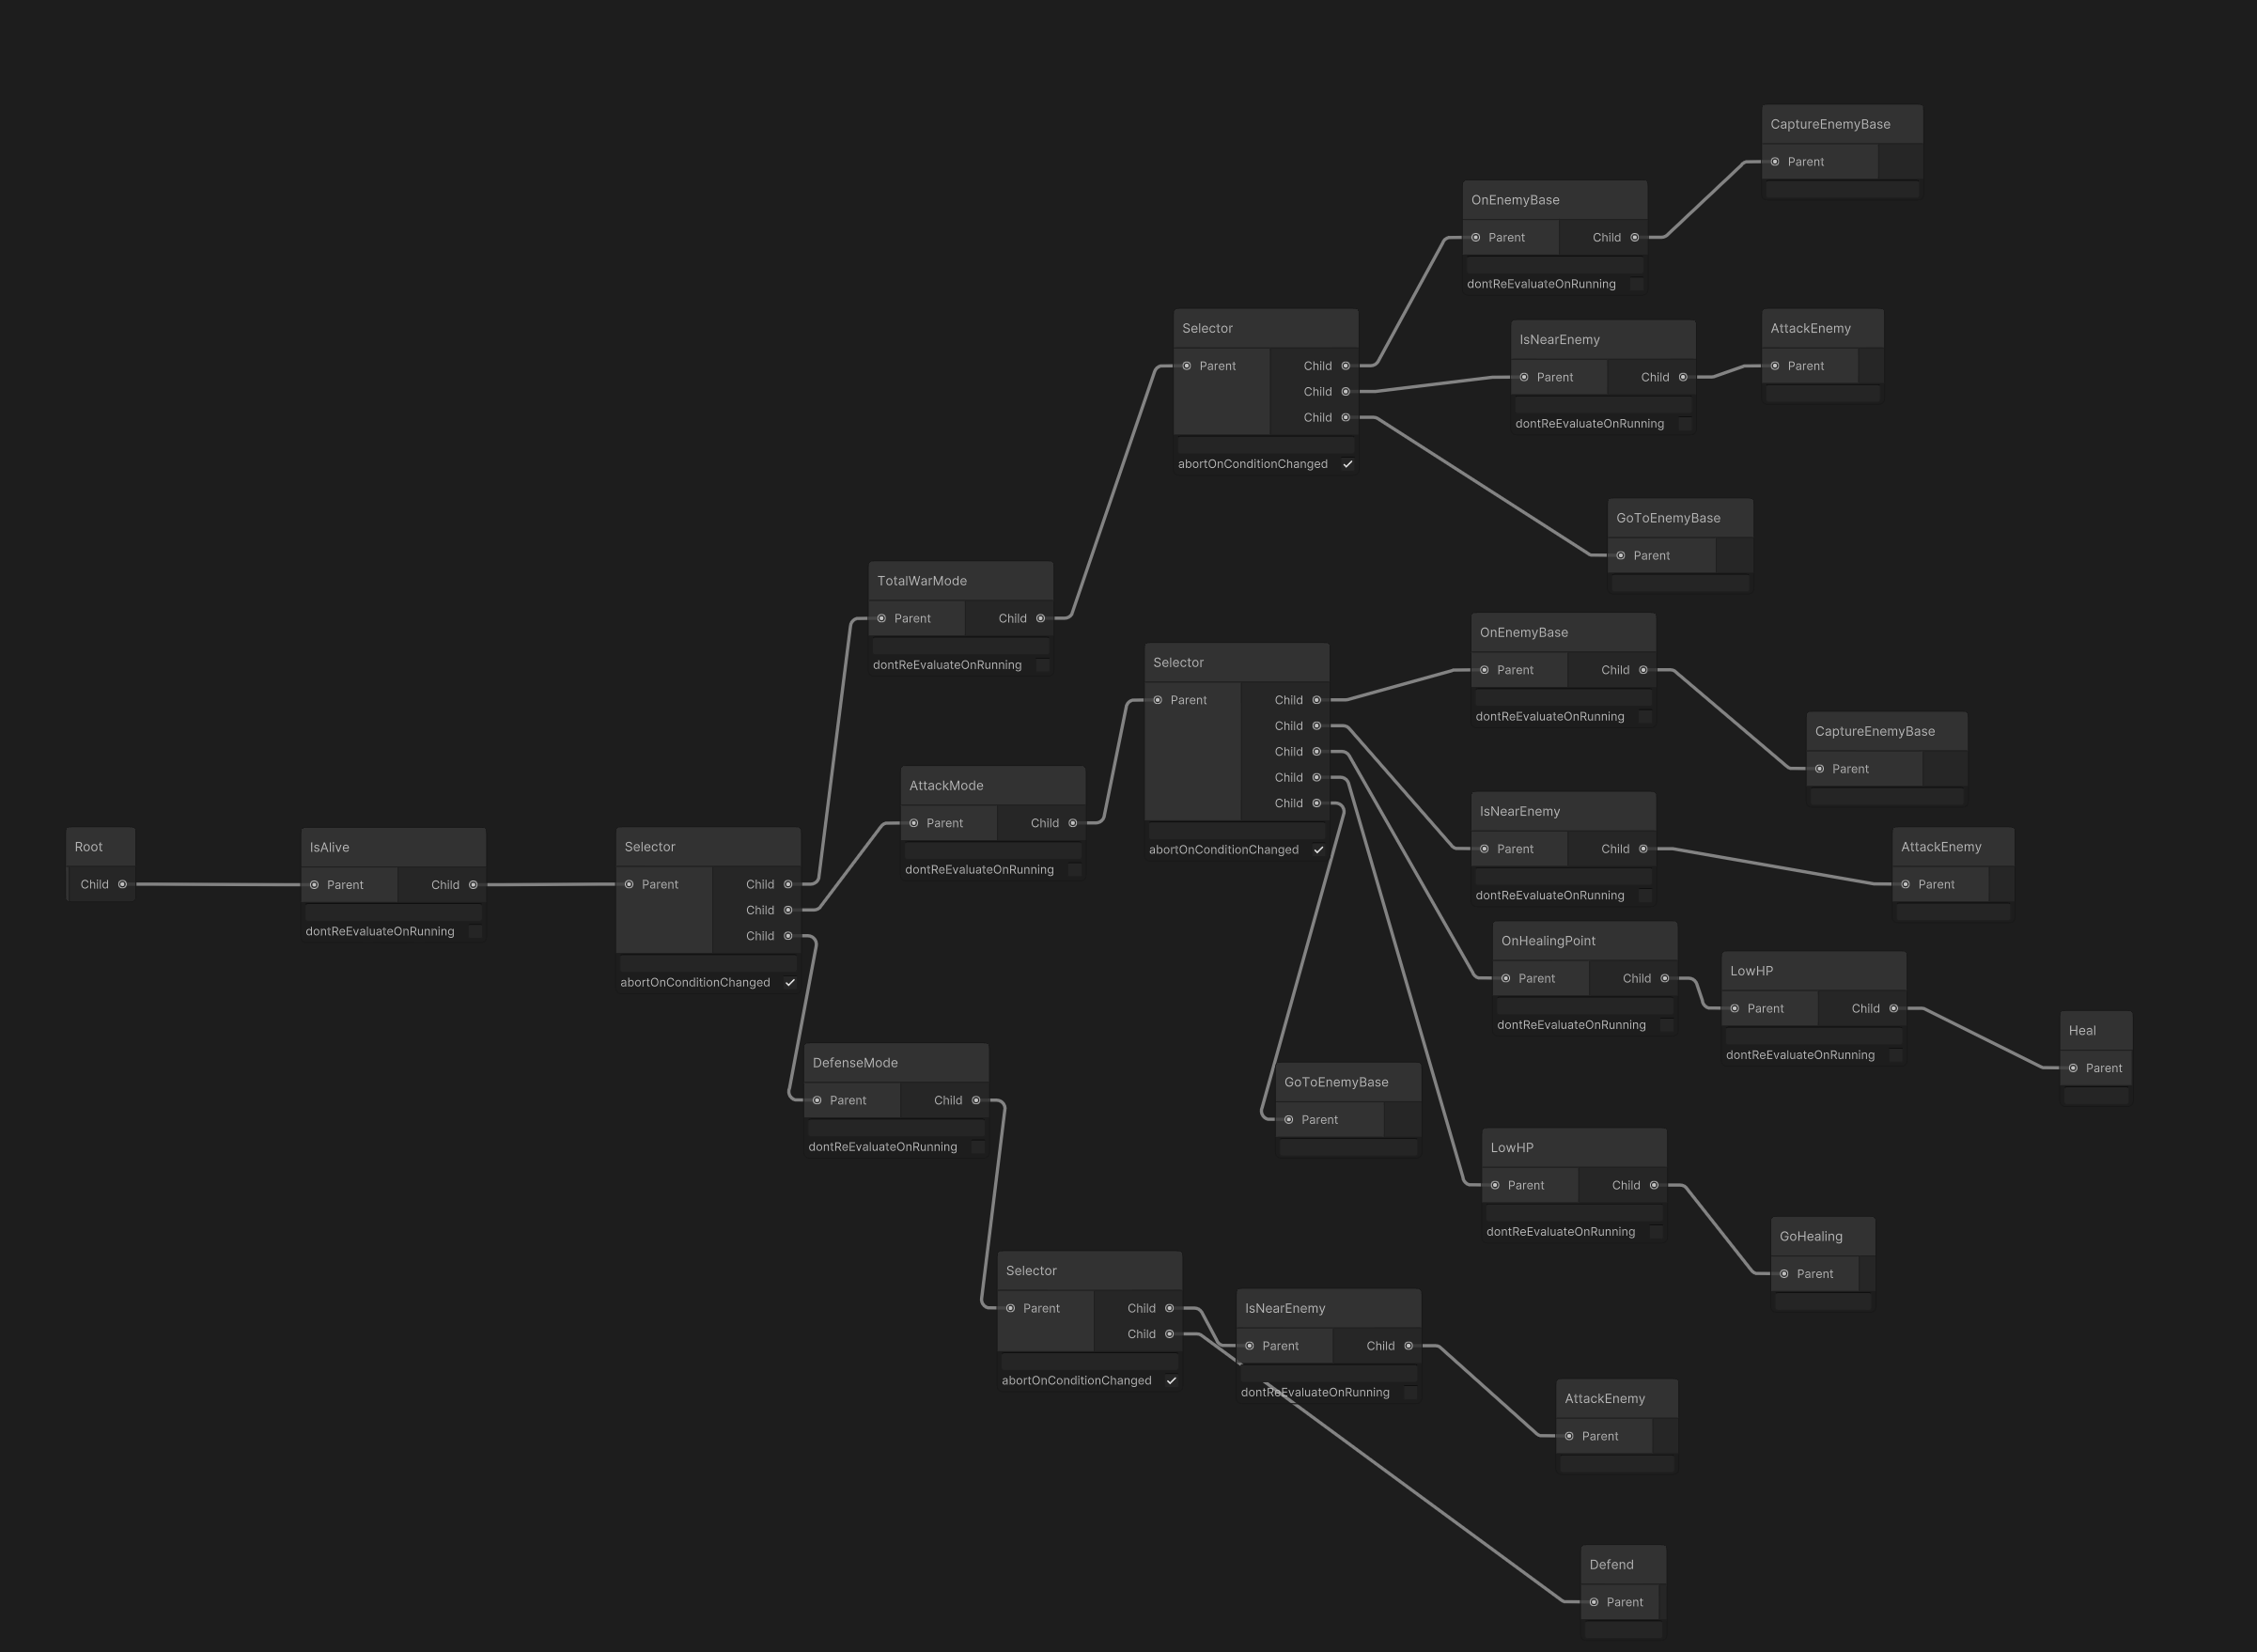
\includegraphics[scale=0.4]{doc/images/ArbolInfanteria.png}
    \caption{Árbol de comportamiento de infantería pesada}
    \label{fig:infantery}
\end{figure}

\subsection{Lancero}
Esta unidad funciona de forma similar a la infantería, solo que la hemos ideado como acompañamiento de esta. En el \textbf{modo ataque} y \textbf{modo guerra total} priorizaran atacar a enemigos antes que capturar, pero siempre priorizan atacar a los enemigos en a la base frente a su salud. En el \textbf{modo defensa} se comportará igual que en la infantería. 
\begin{figure}[H]
    \centering
    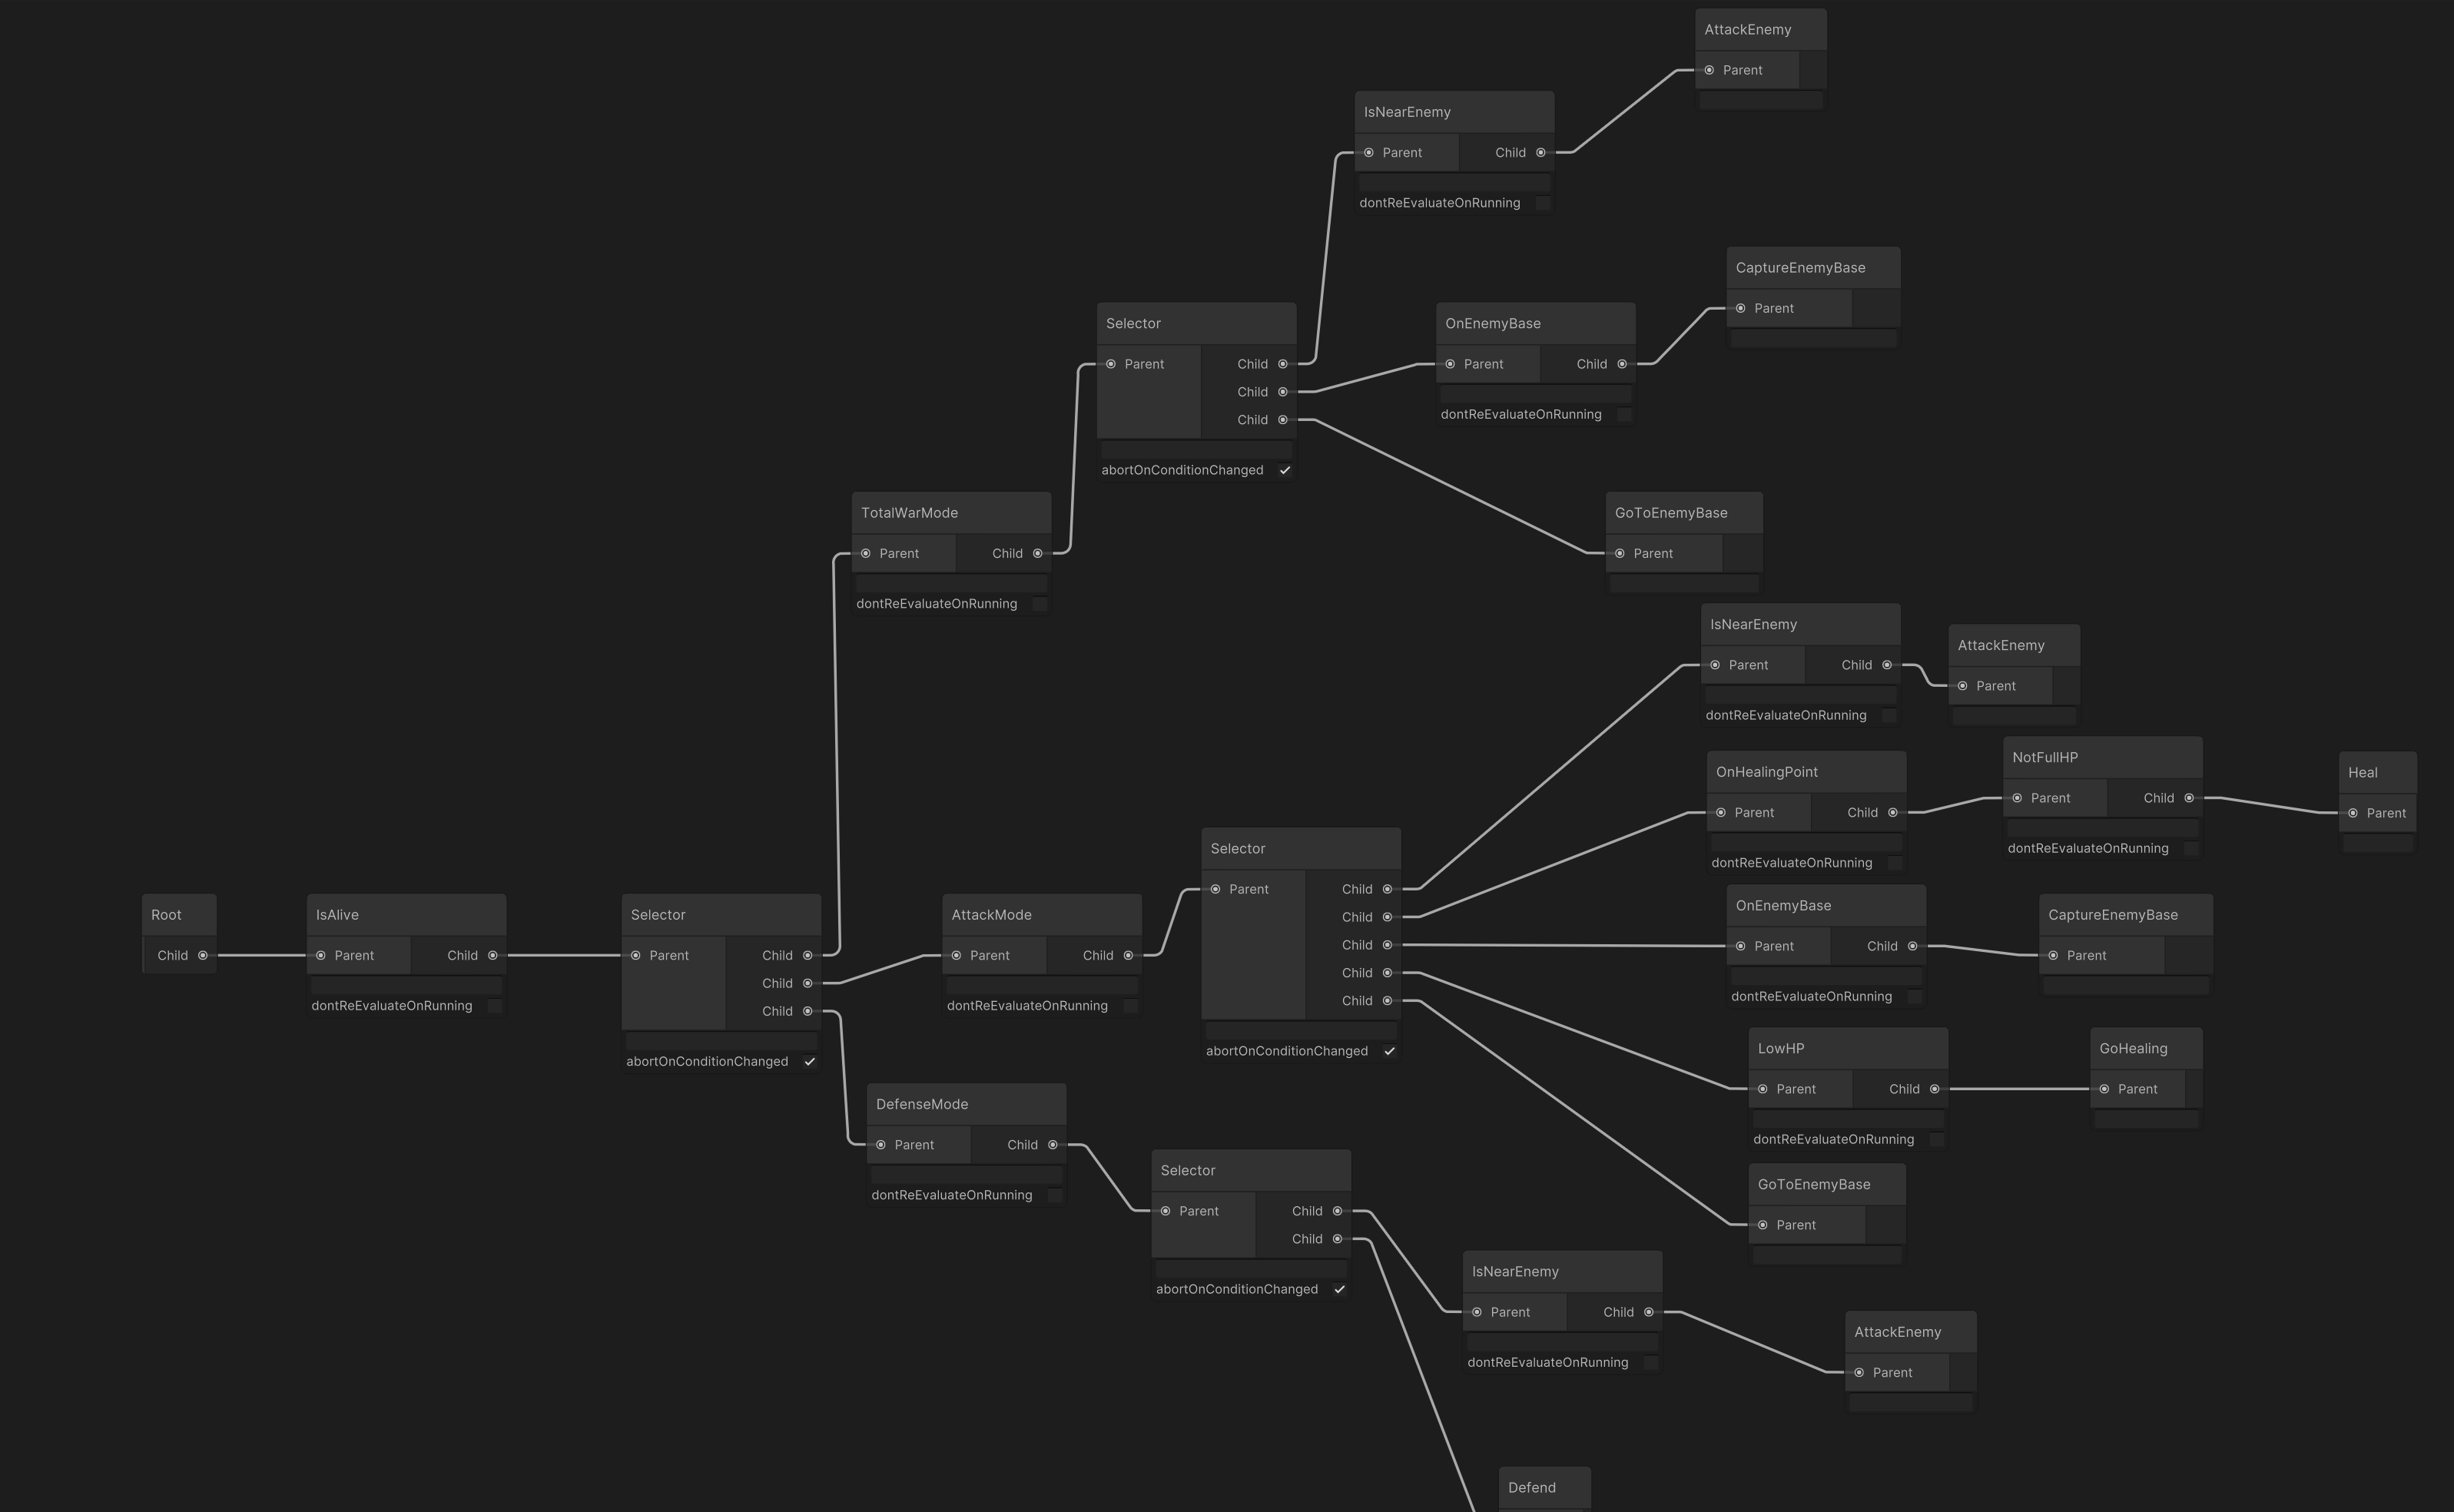
\includegraphics[scale=0.3]{doc/images/ArbolLancero.png}
    \caption{Árbol de comportamiento de lancero}
    \label{fig:lancer}
\end{figure}

\subsection{Arquero}
Para la unidad de tipo arquero, hemos ideado que sea una unidad "cobarde", esta prioriza su vida antes que el trabajo en equipo. A diferencia de las otras unidades esta en el \textbf{modo ataque} buscará atacar y capturar la base enemiga, pero siempre que su vida baje peligrosamente huirá a curarse. En el \textbf{modo defensa} también encontramos esta característica, si la unidad se ve muy dañada, irá a curarse a diferencia de las anteriores unidades que simplemente defendían.

\begin{figure}[H]
    \centering
    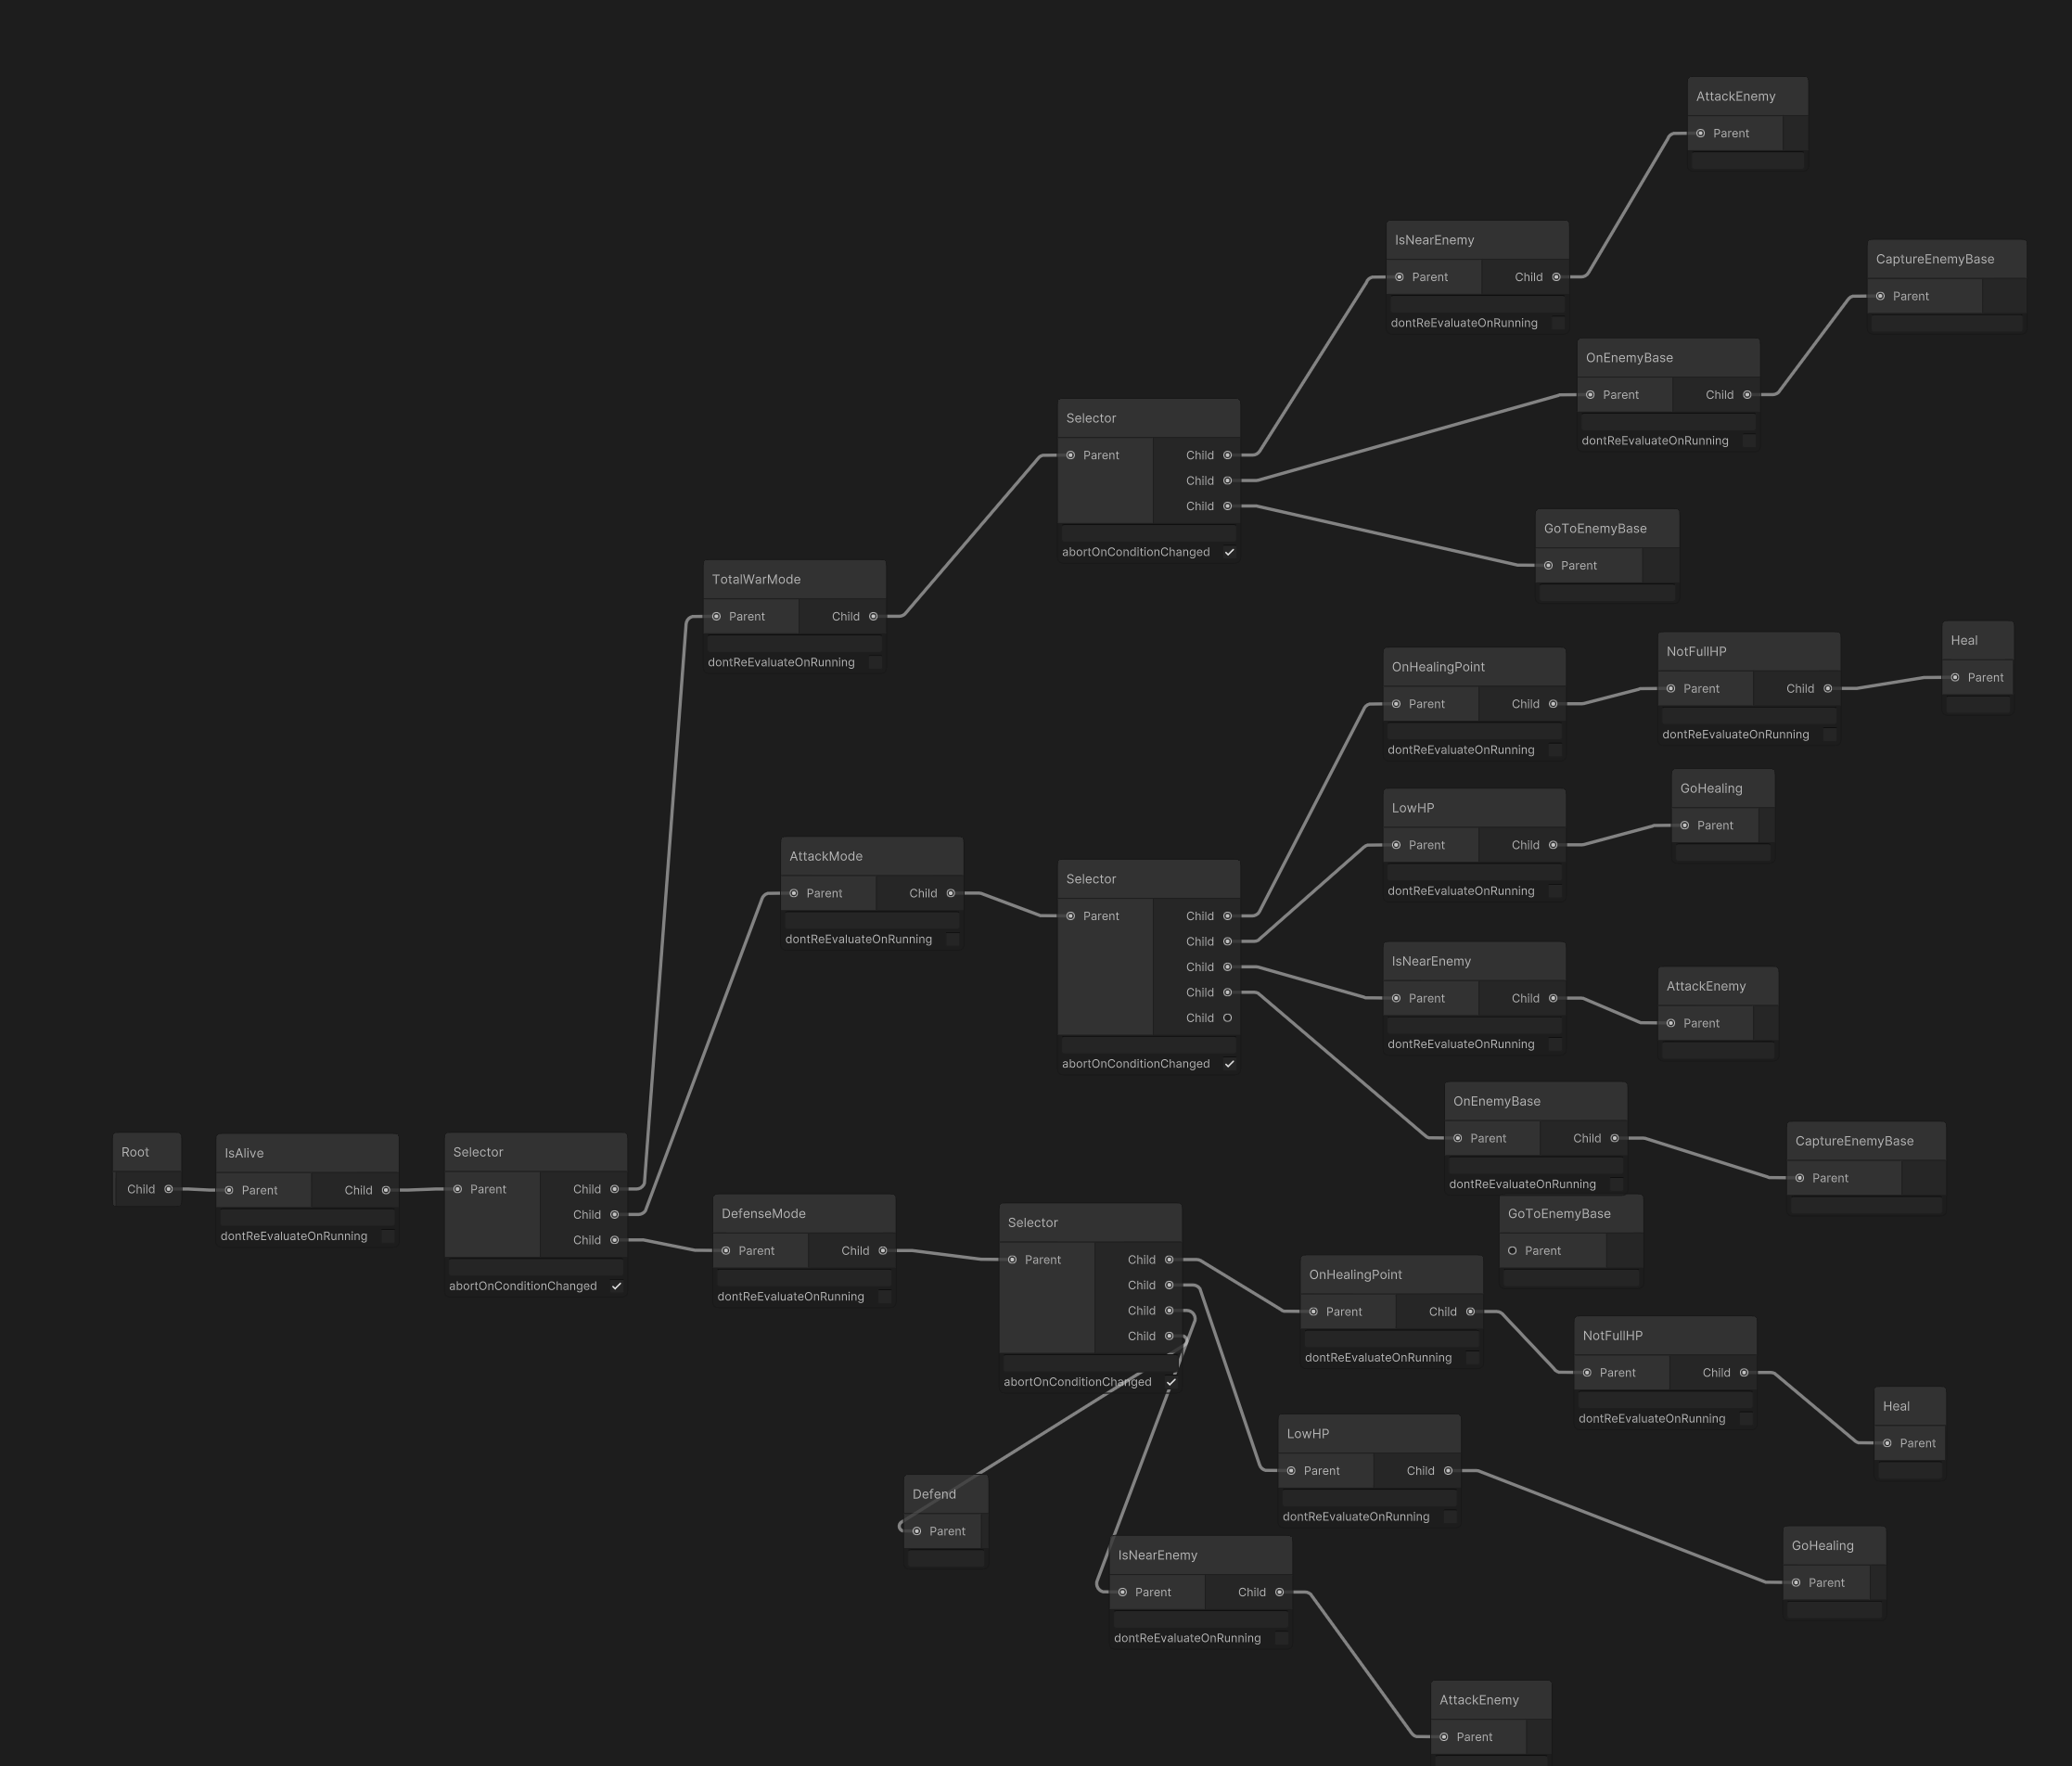
\includegraphics[scale=0.4]{doc/images/ArbolArqueros.png}
    \caption{Árbol de comportamiento de arquero}
    \label{fig:archer}
\end{figure}
\subsection{Caballería} 
Esta unidad la podríamos considerar la mas distintas. de las 4. Su comportamiento se basa en desplazarse en modo de "patrulla" yendo y viniendo a la base. Irá compronbando que se aleje demasiado de su base para volver, y si se encuentra a cualquier enemigo le atacará. Este comportamiendo lo mantendrá siempre que esté \textbf{modo ataque} y en \textbf{modo defensa}. Pero si le ponemos \textbf{modo guerra total} simplemente atacara la base. Cabe recalcar que esta unidad al centrarse en patrullar, nunca llegará a atacar la base enemiga, ni a defender su propia base.

\begin{figure}[H]
    \centering
    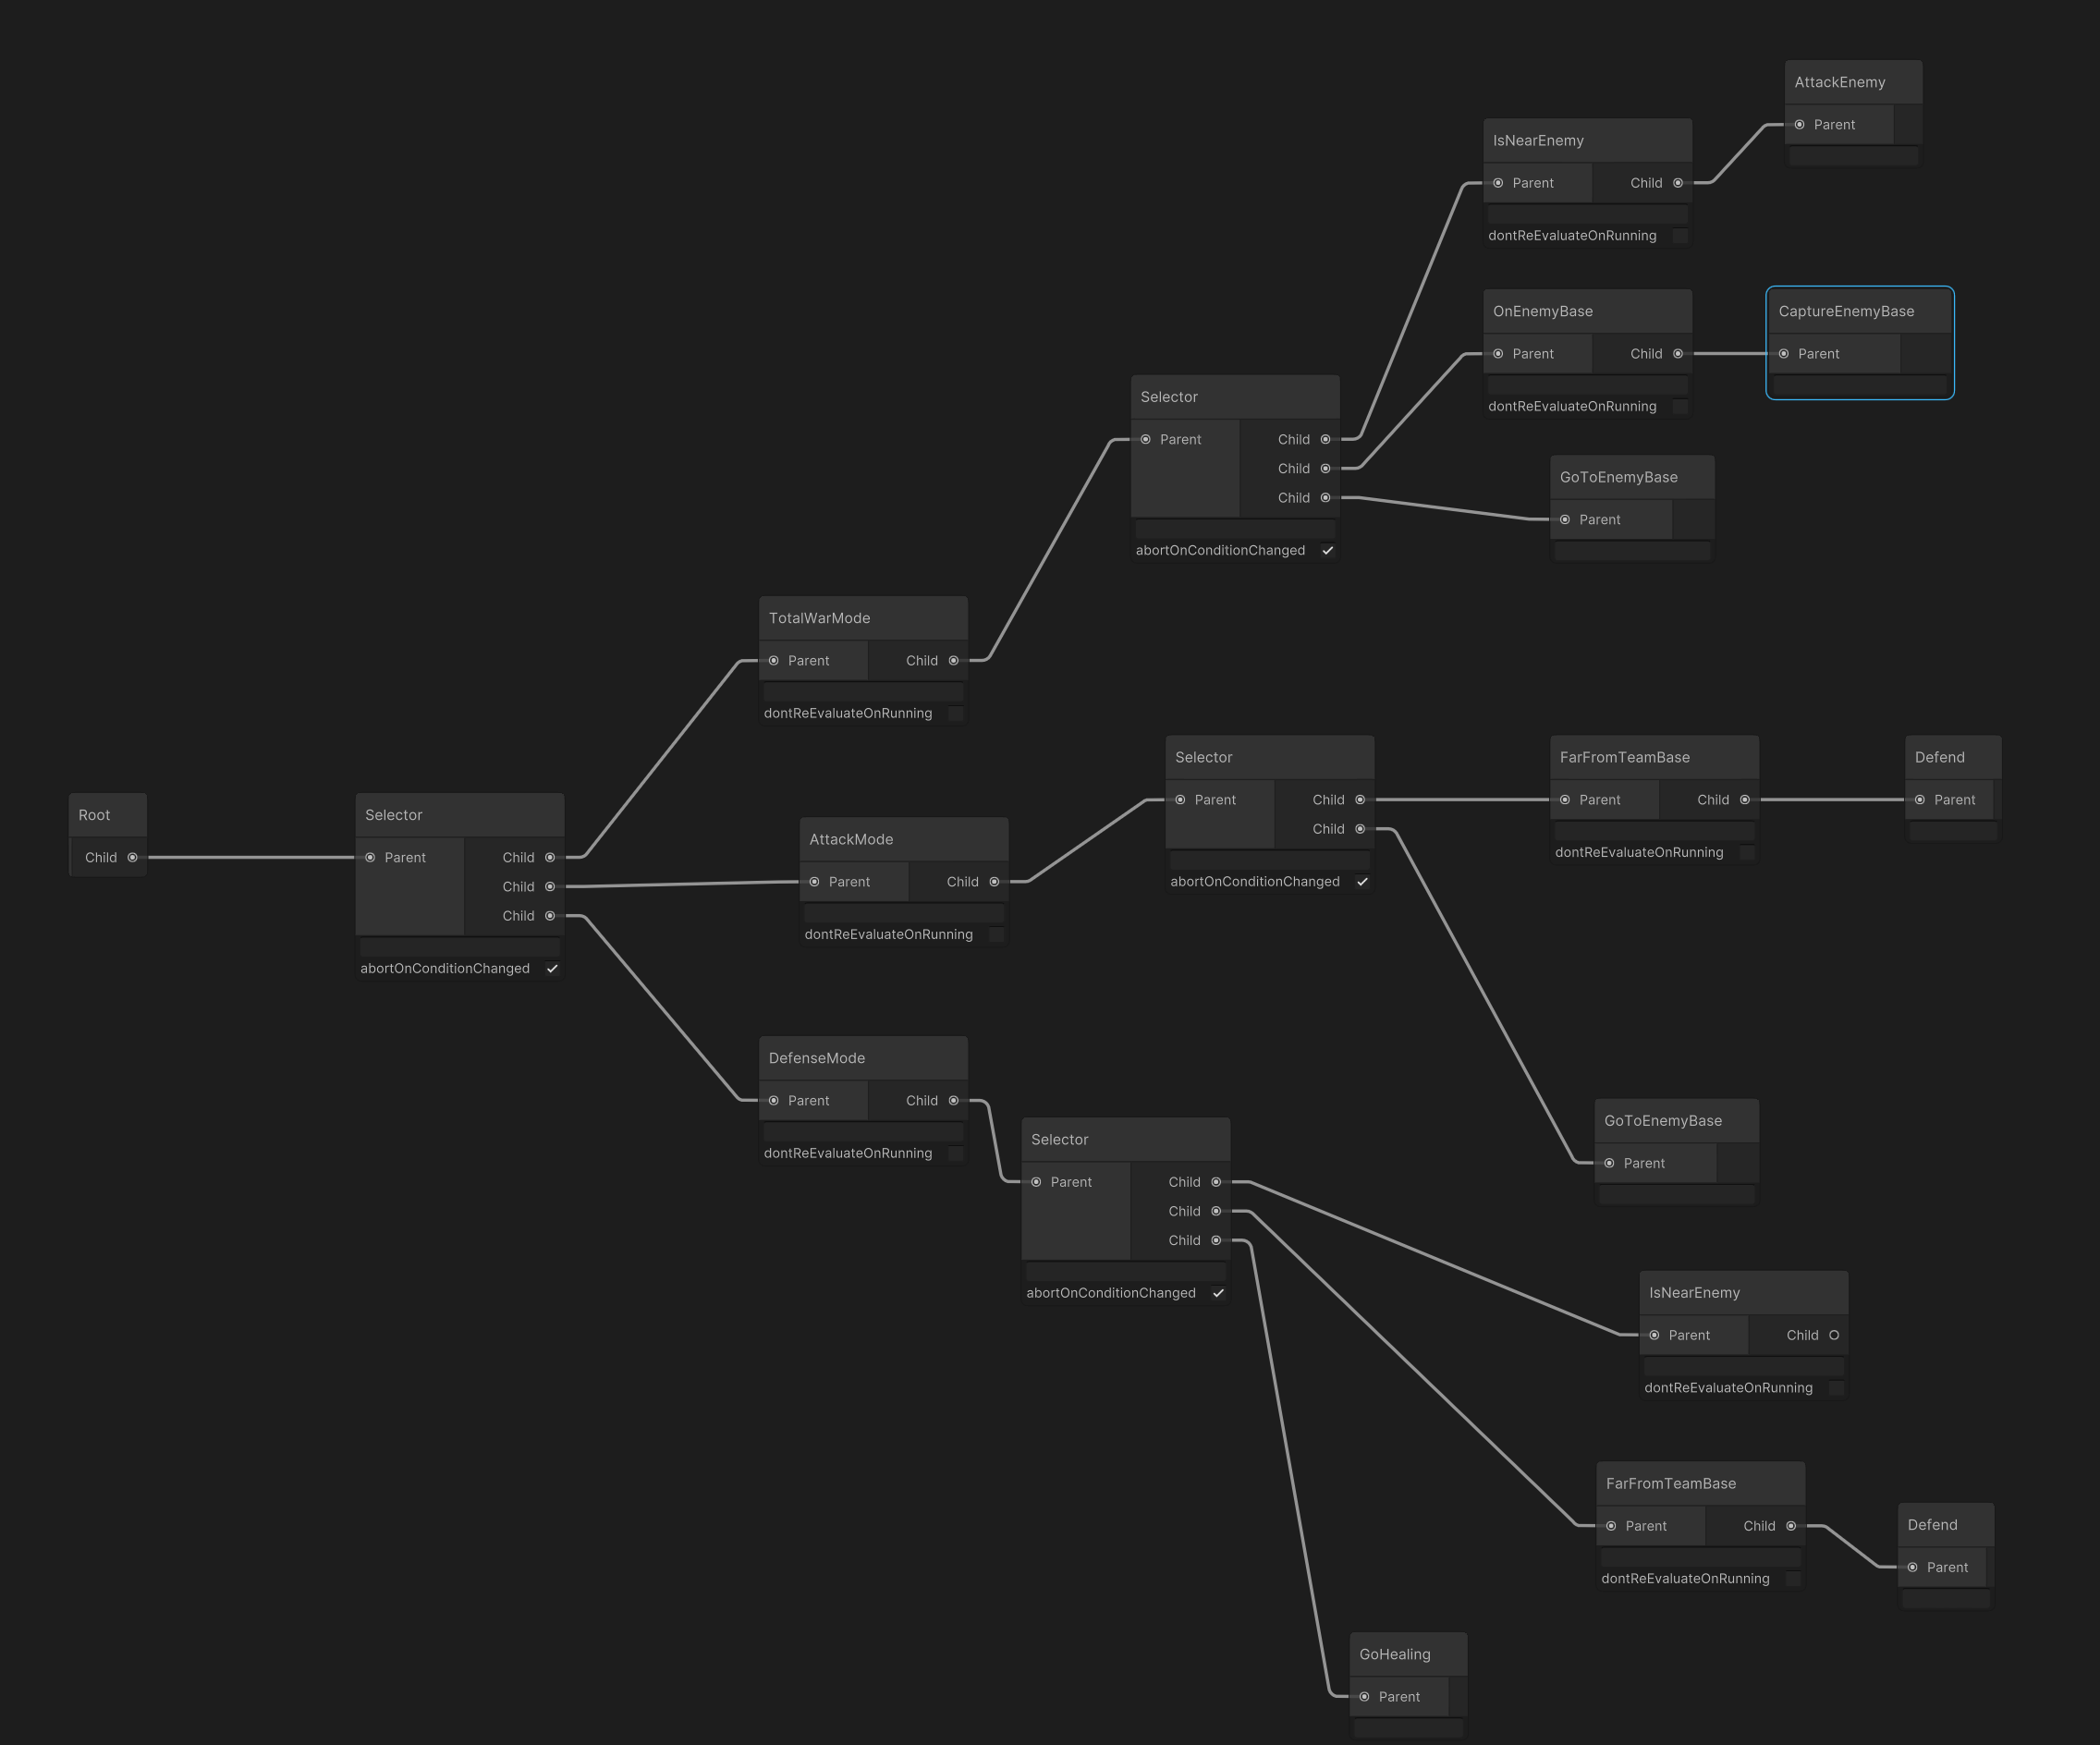
\includegraphics[scale=0.4]{doc/images/ArbolCaballeria.png}
    \caption{Árbol de comportamiento de caballería}
    \label{fig:horse}
\end{figure}
